\documentclass[11pt]{article}
\usepackage[utf8]{inputenc}
\usepackage{geometry}
\geometry{a4paper, margin=1in}
\usepackage{hyperref}
\usepackage{graphicx}
\usepackage{tabularx}
\usepackage{booktabs}
\usepackage{enumitem}
\usepackage{xcolor}
\usepackage{colortbl}
\usepackage{float}
\usepackage{tikz}
\usetikzlibrary{shapes,arrows.meta,positioning,fit,backgrounds,calc,decorations.pathreplacing}

% Colors
\definecolor{oldmethod}{RGB}{255, 220, 220}
\definecolor{ourmethod}{RGB}{210, 240, 210}
\definecolor{limitred}{RGB}{240, 200, 200}
\definecolor{improvgreen}{RGB}{200, 240, 200}

\title{Comparison of Result 0 (Baseline) with Previous Research Models\\[0.3em]
\large Landslide Identification Using Machine Learning}
\author{}
\date{2026-03-17}

\begin{document}

\maketitle
\tableofcontents
\newpage

% ============================================================================
\section{Introduction}
% ============================================================================

Before our project, several approaches existed for identifying landslides from satellite imagery and geospatial data. Each had significant limitations. This document compares our \textbf{Result 0 (r0)} --- the baseline AlexNet + HMM two-phase pipeline --- against these prior methods, highlighting what they could and could not do, and how our architecture addresses their gaps.

Our r0 system already surpasses most prior methods in a critical way: it combines \textbf{image-based detection} (Phase 1) with \textbf{temporal type prediction and forecasting} (Phase 2) in a single automated pipeline. No previous publicly available system did both.

% ============================================================================
\section{Previous Research Models --- Overview}
% ============================================================================

The landslide detection literature can be grouped into four broad categories:

\begin{enumerate}
    \item \textbf{Remote Sensing Index Methods} --- NDVI, change detection, spectral analysis.
    \item \textbf{Classical Machine Learning on Engineered Features} --- SVM, Random Forest on terrain data.
    \item \textbf{Deep Learning Segmentation} --- U-Net, ResNet on pixel-level masks.
    \item \textbf{Sequential / Temporal Models} --- LSTM, GRU on event time-series.
\end{enumerate}

% ============================================================================
\section{Previous Architecture Flowcharts}
% ============================================================================

\subsection{Method 1: NDVI / Change Detection Approach}

This is the simplest and oldest approach. Satellite images from two time points (before and after a suspected event) are compared using vegetation indices like NDVI. Areas where vegetation dropped sharply are flagged as potential landslides.

\begin{figure}[H]
\centering
\resizebox{0.85\textwidth}{!}{
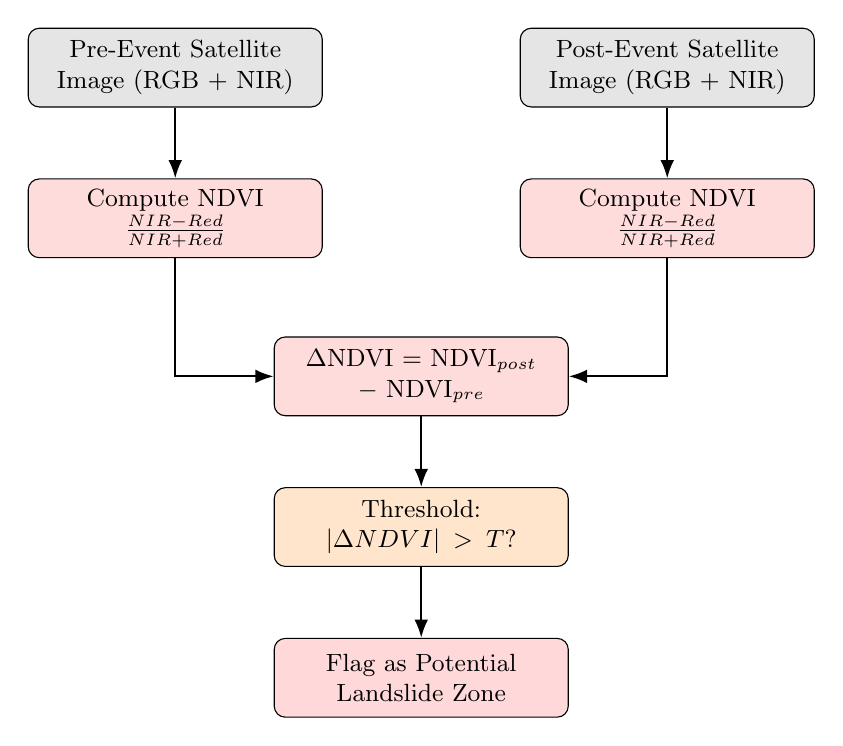
\begin{tikzpicture}[
    node distance=0.9cm and 1.5cm,
    box/.style={draw, rectangle, rounded corners, align=center, fill=oldmethod, text width=3.5cm, minimum height=1cm, font=\small},
    arrow/.style={-Latex, thick}
]
    \node[box, fill=gray!20] (pre) {Pre-Event Satellite\\Image (RGB + NIR)};
    \node[box, fill=gray!20, right=2.5cm of pre] (post) {Post-Event Satellite\\Image (RGB + NIR)};

    \node[box, below=of pre] (ndvi1) {Compute NDVI\\$\frac{\text{NIR} - \text{Red}}{\text{NIR} + \text{Red}}$};
    \node[box, below=of post] (ndvi2) {Compute NDVI\\$\frac{\text{NIR} - \text{Red}}{\text{NIR} + \text{Red}}$};

    \node[box, below=1.5cm of $(ndvi1)!0.5!(ndvi2)$] (diff) {$\Delta$NDVI = NDVI$_{\text{post}}$ $-$ NDVI$_{\text{pre}}$};

    \node[box, below=of diff, fill=orange!20] (thresh) {Threshold:\\$|\Delta\text{NDVI}| > T$?};

    \node[box, below=of thresh, fill=red!15] (out) {Flag as Potential\\Landslide Zone};

    \draw[arrow] (pre) -- (ndvi1);
    \draw[arrow] (post) -- (ndvi2);
    \draw[arrow] (ndvi1) |- (diff);
    \draw[arrow] (ndvi2) |- (diff);
    \draw[arrow] (diff) -- (thresh);
    \draw[arrow] (thresh) -- (out);
\end{tikzpicture}
}
\caption{NDVI / Change Detection pipeline. Requires \emph{two} images (before and after) and only detects vegetation loss, not landslide type.}
\end{figure}

\textbf{Limitations:}
\begin{itemize}[nosep]
    \item Requires a \emph{before} image --- useless if no pre-event data exists.
    \item Only detects vegetation change, not landslides specifically (deforestation, fire, and agriculture also reduce NDVI).
    \item Cannot classify the \emph{type} of landslide.
    \item No temporal forecasting capability.
    \item Requires manual threshold tuning per region.
\end{itemize}

% ---

\subsection{Method 2: SVM / Random Forest on Terrain Features}

These methods extract handcrafted features from Digital Elevation Models (DEMs) and land-cover maps --- slope angle, aspect, elevation, lithology, soil type, proximity to rivers, rainfall --- and feed them into a classical classifier.

\begin{figure}[H]
\centering
\resizebox{0.9\textwidth}{!}{
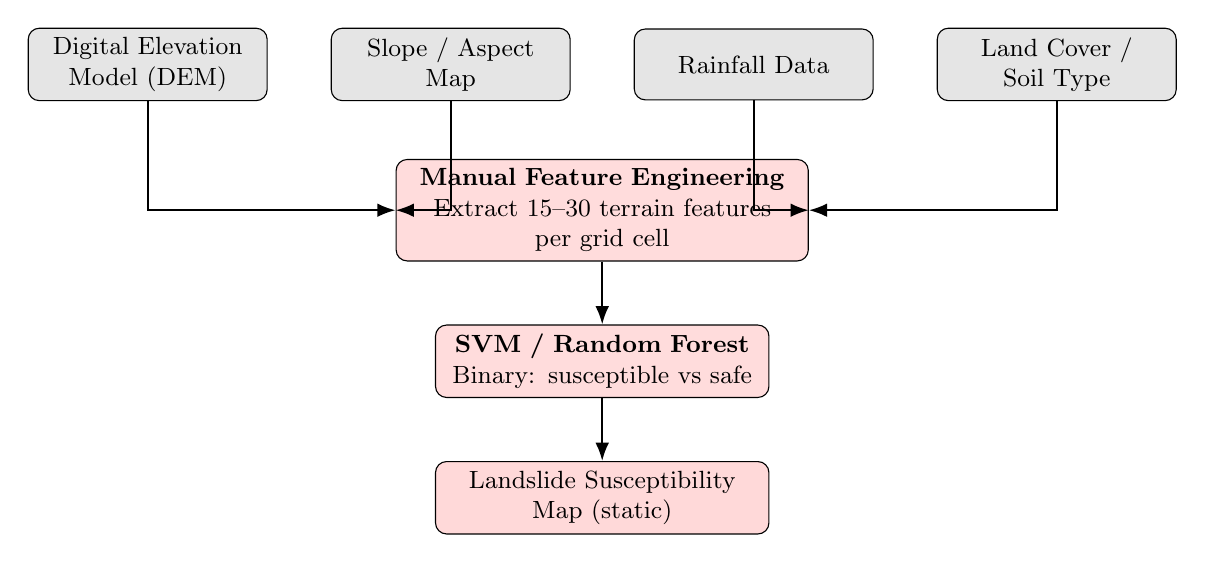
\begin{tikzpicture}[
    node distance=0.8cm and 0.8cm,
    box/.style={draw, rectangle, rounded corners, align=center, fill=oldmethod, text width=2.8cm, minimum height=0.9cm, font=\small},
    arrow/.style={-Latex, thick}
]
    % Input features
    \node[box, fill=gray!20] (dem) {Digital Elevation\\Model (DEM)};
    \node[box, fill=gray!20, right=of dem] (slope) {Slope / Aspect\\Map};
    \node[box, fill=gray!20, right=of slope] (rain) {Rainfall Data};
    \node[box, fill=gray!20, right=of rain] (lc) {Land Cover /\\Soil Type};

    % Feature engineering
    \node[box, below=1.2cm of $(dem)!0.5!(lc)$, text width=5cm] (feat) {\textbf{Manual Feature Engineering}\\Extract 15--30 terrain features\\per grid cell};

    % Classifier
    \node[box, below=of feat, text width=4cm] (svm) {\textbf{SVM / Random Forest}\\Binary: susceptible vs safe};

    % Output
    \node[box, below=of svm, fill=red!15, text width=4cm] (map) {Landslide Susceptibility\\Map (static)};

    \draw[arrow] (dem) |- (feat);
    \draw[arrow] (slope) |- (feat);
    \draw[arrow] (rain) |- (feat);
    \draw[arrow] (lc) |- (feat);
    \draw[arrow] (feat) -- (svm);
    \draw[arrow] (svm) -- (map);
\end{tikzpicture}
}
\caption{SVM / Random Forest susceptibility mapping. Requires manual feature engineering and produces only static maps.}
\end{figure}

\textbf{Limitations:}
\begin{itemize}[nosep]
    \item Requires \emph{manual feature engineering} by domain experts for each new region.
    \item Does not process raw satellite images --- cannot detect visual anomalies.
    \item Produces a \emph{static} susceptibility map, not a dynamic detection system.
    \item Cannot generalize across different geographies without re-engineering features.
    \item No temporal prediction or forecasting.
\end{itemize}

% ---

\subsection{Method 3: U-Net / ResNet Deep Learning Segmentation}

Modern deep learning approaches apply encoder-decoder architectures (like U-Net) or deep classification networks (like ResNet-50) to satellite imagery for pixel-level segmentation or patch-level classification.

\begin{figure}[H]
\centering
\resizebox{0.85\textwidth}{!}{
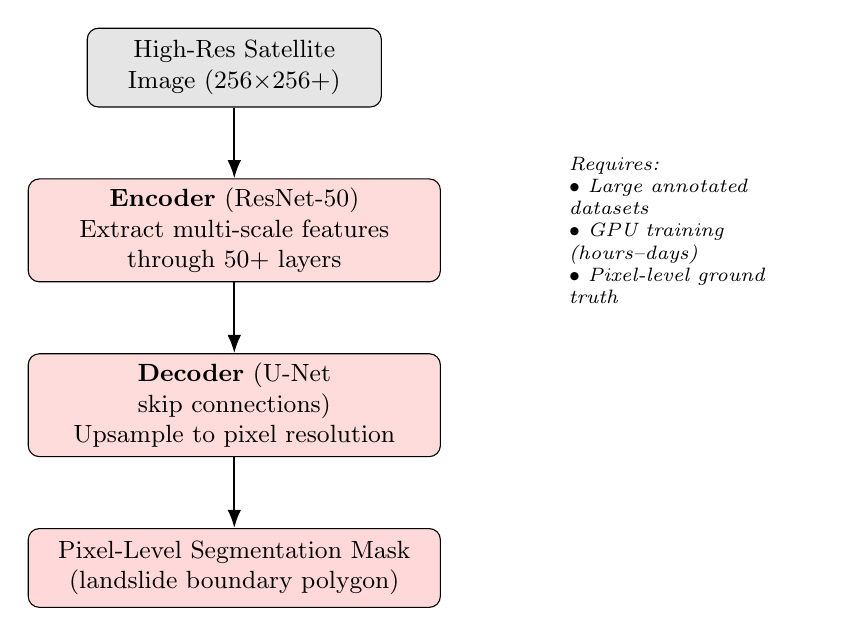
\begin{tikzpicture}[
    node distance=0.9cm,
    box/.style={draw, rectangle, rounded corners, align=center, fill=oldmethod, text width=3.5cm, minimum height=1cm, font=\small},
    arrow/.style={-Latex, thick}
]
    \node[box, fill=gray!20] (input) {High-Res Satellite\\Image (256$\times$256+)};

    \node[box, below=of input, text width=5cm] (enc) {\textbf{Encoder} (ResNet-50)\\Extract multi-scale features\\through 50+ layers};

    \node[box, below=of enc, text width=5cm] (dec) {\textbf{Decoder} (U-Net skip connections)\\Upsample to pixel resolution};

    \node[box, below=of dec, fill=red!15, text width=5cm] (mask) {Pixel-Level Segmentation Mask\\(landslide boundary polygon)};

    \draw[arrow] (input) -- (enc);
    \draw[arrow] (enc) -- (dec);
    \draw[arrow] (dec) -- (mask);

    \node[right=1.5cm of enc, text width=3cm, font=\scriptsize\itshape, align=left] {Requires:\\$\bullet$ Large annotated datasets\\$\bullet$ GPU training (hours--days)\\$\bullet$ Pixel-level ground truth};
\end{tikzpicture}
}
\caption{U-Net / ResNet segmentation pipeline. Powerful but requires massive labelled data and has no temporal component.}
\end{figure}

\textbf{Limitations:}
\begin{itemize}[nosep]
    \item Requires \emph{very large annotated datasets} with pixel-level masks (expensive to create).
    \item Only performs detection at the moment of the image --- no prediction of \emph{future} events.
    \item Cannot classify the \emph{type} of landslide (only ``landslide vs background'').
    \item No integration with historical event data for risk assessment.
    \item Computationally expensive --- requires high-end GPUs and hours of training.
\end{itemize}

% ---

\subsection{Method 4: LSTM / GRU Temporal Models}

Recurrent neural networks like LSTM and GRU can learn temporal patterns in sequences of landslide events to predict future occurrences.

\begin{figure}[H]
\centering
\resizebox{0.85\textwidth}{!}{
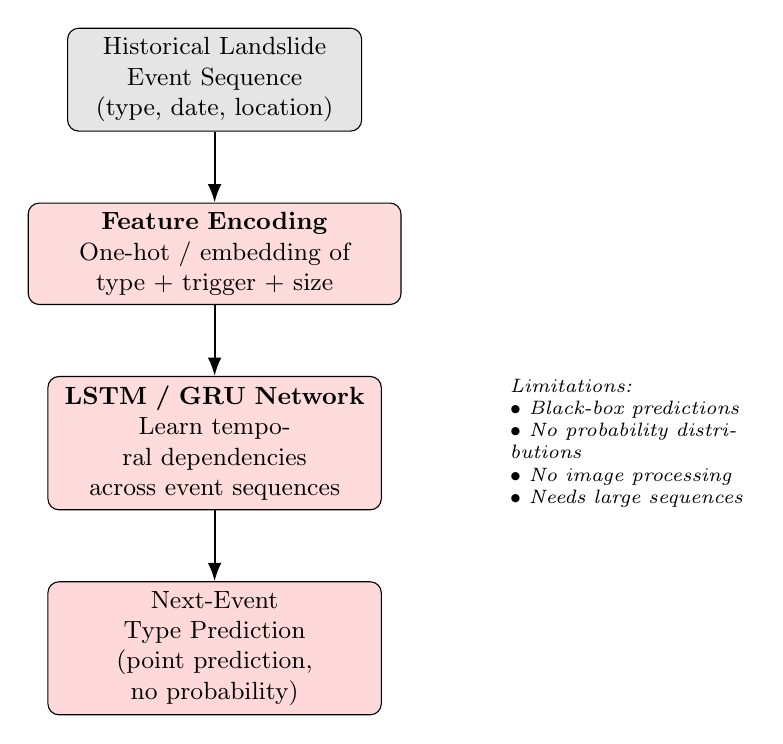
\begin{tikzpicture}[
    node distance=0.9cm,
    box/.style={draw, rectangle, rounded corners, align=center, fill=oldmethod, text width=3.5cm, minimum height=1cm, font=\small},
    arrow/.style={-Latex, thick}
]
    \node[box, fill=gray!20] (data) {Historical Landslide\\Event Sequence\\(type, date, location)};

    \node[box, below=of data, text width=4.5cm] (embed) {\textbf{Feature Encoding}\\One-hot / embedding of\\type + trigger + size};

    \node[box, below=of embed, text width=4cm] (lstm) {\textbf{LSTM / GRU Network}\\Learn temporal dependencies\\across event sequences};

    \node[box, below=of lstm, fill=red!15, text width=4cm] (pred) {Next-Event Type Prediction\\(point prediction, no probability)};

    \draw[arrow] (data) -- (embed);
    \draw[arrow] (embed) -- (lstm);
    \draw[arrow] (lstm) -- (pred);

    \node[right=1.5cm of lstm, text width=3cm, font=\scriptsize\itshape, align=left] {Limitations:\\$\bullet$ Black-box predictions\\$\bullet$ No probability distributions\\$\bullet$ No image processing\\$\bullet$ Needs large sequences};
\end{tikzpicture}
}
\caption{LSTM / GRU temporal prediction pipeline. No image analysis; produces point predictions without probabilities.}
\end{figure}

\textbf{Limitations:}
\begin{itemize}[nosep]
    \item Does not process satellite images --- purely event-sequence based.
    \item Produces point predictions (``next type = Rockfall'') with no probability distribution.
    \item Black-box model --- transition dynamics are not interpretable.
    \item Requires large sequential datasets to avoid overfitting.
    \item Cannot provide occurrence probability or peak risk month.
\end{itemize}

% ============================================================================
\newpage
\section{Our Architecture: Result 0 (AlexNet + HMM)}
% ============================================================================

\begin{figure}[H]
\centering
\resizebox{0.95\textwidth}{!}{
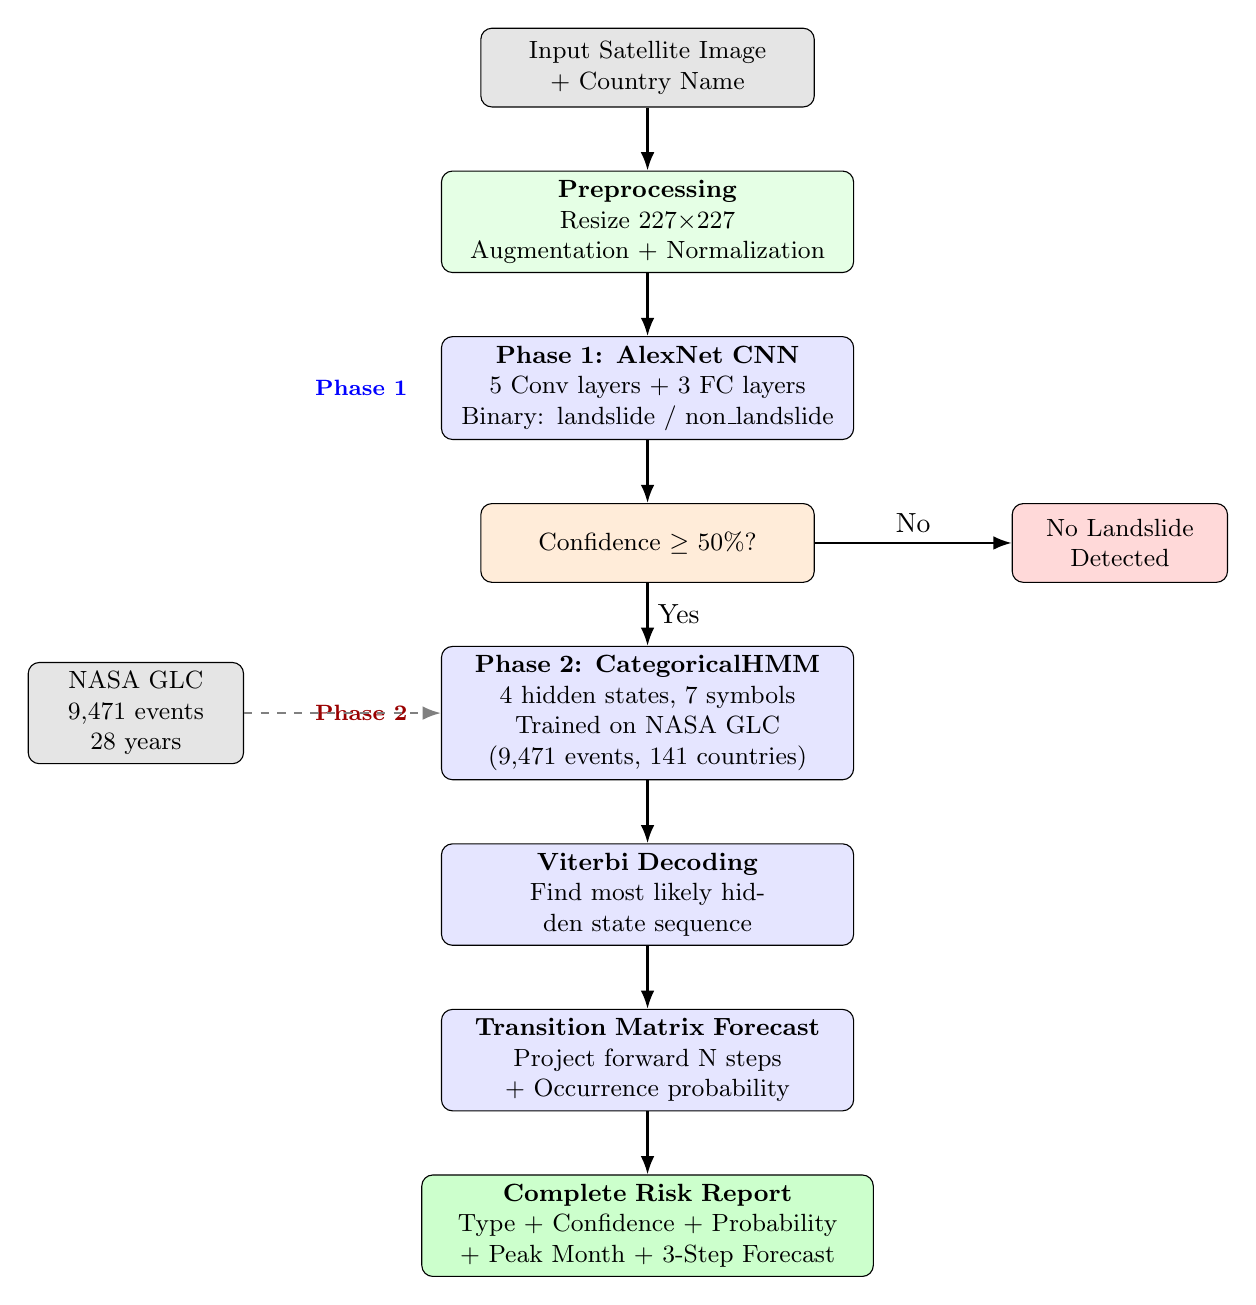
\begin{tikzpicture}[
    node distance=0.8cm and 1.2cm,
    box/.style={draw, rectangle, rounded corners, align=center, fill=ourmethod, text width=3.5cm, minimum height=1cm, font=\small},
    arrow/.style={-Latex, thick}
]
    % Inputs
    \node[box, fill=gray!20, text width=4cm] (input) {Input Satellite Image\\+ Country Name};

    % Preprocessing
    \node[box, below=of input, fill=green!10, text width=5cm] (pre) {\textbf{Preprocessing}\\Resize 227$\times$227\\Augmentation + Normalization};

    % Phase 1
    \node[box, below=of pre, text width=5cm, fill=blue!10] (alex) {\textbf{Phase 1: AlexNet CNN}\\5 Conv layers + 3 FC layers\\Binary: landslide / non\_landslide};

    \node[box, below=of alex, fill=orange!15, text width=4cm] (dec) {Confidence $\geq$ 50\%?};

    % Phase 2
    \node[box, below=of dec, text width=5cm, fill=blue!10] (hmm) {\textbf{Phase 2: CategoricalHMM}\\4 hidden states, 7 symbols\\Trained on NASA GLC\\(9,471 events, 141 countries)};

    \node[box, below=of hmm, text width=5cm, fill=blue!10] (viterbi) {\textbf{Viterbi Decoding}\\Find most likely hidden state sequence};

    \node[box, below=of viterbi, text width=5cm, fill=blue!10] (forecast) {\textbf{Transition Matrix Forecast}\\Project forward N steps\\+ Occurrence probability};

    % Output
    \node[box, below=of forecast, fill=green!20, text width=5.5cm] (out) {\textbf{Complete Risk Report}\\Type + Confidence + Probability\\+ Peak Month + 3-Step Forecast};

    % No branch
    \node[box, right=2.5cm of dec, fill=red!15, text width=2.5cm] (no) {No Landslide\\Detected};

    % Connections
    \draw[arrow] (input) -- (pre);
    \draw[arrow] (pre) -- (alex);
    \draw[arrow] (alex) -- (dec);
    \draw[arrow] (dec) -- node[right] {Yes} (hmm);
    \draw[arrow] (dec) -- node[above] {No} (no);
    \draw[arrow] (hmm) -- (viterbi);
    \draw[arrow] (viterbi) -- (forecast);
    \draw[arrow] (forecast) -- (out);

    % Phase labels
    \node[left=0.3cm of alex, font=\footnotesize\bfseries, blue] {Phase 1};
    \node[left=0.3cm of hmm, font=\footnotesize\bfseries, red!60!black] {Phase 2};

    % NASA GLC data input
    \node[box, fill=gray!20, left=2.5cm of hmm, text width=2.5cm] (nasa) {NASA GLC\\9,471 events\\28 years};
    \draw[arrow, dashed, gray] (nasa) -- (hmm);
\end{tikzpicture}
}
\caption{Our r0 pipeline: AlexNet (image detection) + HMM (temporal forecasting). Green background = our system.}
\end{figure}

% ============================================================================
\section{Side-by-Side Comparison Table}
% ============================================================================

\begin{table}[H]
\centering
\footnotesize
\resizebox{\textwidth}{!}{
\begin{tabular}{@{}p{2.8cm}ccccc@{}}
\toprule
\textbf{Capability} &
\textbf{NDVI/Change} &
\textbf{SVM/RF} &
\textbf{U-Net/ResNet} &
\textbf{LSTM/GRU} &
\cellcolor{improvgreen}\textbf{Our r0 (AlexNet+HMM)} \\
\midrule
Processes raw images & No (index only) & No (features) & \textbf{Yes} & No & \cellcolor{improvgreen}\textbf{Yes} \\
Single-image detection & No (needs pair) & No (static map) & \textbf{Yes} & No & \cellcolor{improvgreen}\textbf{Yes} \\
Predicts landslide type & No & No & No & Yes & \cellcolor{improvgreen}\textbf{Yes} \\
Future forecasting & No & No & No & Partial & \cellcolor{improvgreen}\textbf{Yes (3-step)} \\
Occurrence probability & No & No & No & No & \cellcolor{improvgreen}\textbf{Yes} \\
Peak risk month & No & No & No & No & \cellcolor{improvgreen}\textbf{Yes} \\
Country risk profile & No & No & No & No & \cellcolor{improvgreen}\textbf{Yes} \\
Interpretable temporal model & N/A & N/A & N/A & No (black-box) & \cellcolor{improvgreen}\textbf{Yes (transition matrix)} \\
Needs manual features & Yes (threshold) & \textbf{Yes (15--30)} & No & Partial & \cellcolor{improvgreen}No \\
Needs before/after pair & \textbf{Yes} & No & No & No & \cellcolor{improvgreen}No \\
Needs pixel-level masks & No & No & \textbf{Yes} & No & \cellcolor{improvgreen}No \\
Training data needed & Low & Medium & \textbf{Very high} & High & \cellcolor{improvgreen}Medium (2,190 images) \\
Training time & Minutes & Minutes & Hours--days & Hours & \cellcolor{improvgreen}$\sim$30 min (GPU) \\
\bottomrule
\end{tabular}
}
\caption{Feature comparison: previous methods vs our r0 baseline. Green cells = our system's advantage.}
\end{table}

% ============================================================================
\section{Performance Comparison}
% ============================================================================

Direct numerical comparison is difficult because most prior studies use different datasets, different definitions of ``landslide,'' and different evaluation protocols. However, we can compare typical reported ranges from the literature:

\begin{table}[H]
\centering
\footnotesize
\begin{tabular}{@{}llcccl@{}}
\toprule
\textbf{Method} & \textbf{Typical Study} & \textbf{Accuracy} & \textbf{F1} & \textbf{AUC} & \textbf{Notes} \\
\midrule
NDVI thresholding & Mondini et al.\ (2011) & 70--80\% & N/A & N/A & Requires image pairs \\
SVM on DEM features & Yilmaz (2010) & 75--85\% & 0.60--0.72 & 0.80--0.87 & Static susceptibility only \\
Random Forest terrain & Catani et al.\ (2013) & 78--88\% & 0.65--0.78 & 0.82--0.90 & Region-specific features \\
ResNet-50 classification & Ghorbanzadeh et al.\ (2019) & 82--90\% & 0.75--0.85 & 0.88--0.94 & Large dataset required \\
U-Net segmentation & Prakash et al.\ (2021) & 85--92\% & 0.78--0.88 & 0.90--0.95 & Pixel-level masks needed \\
LSTM event prediction & Sameen et al.\ (2020) & N/A & 0.70--0.80 & N/A & No image processing \\
\midrule
\rowcolor{improvgreen}
\textbf{Our r0 (AlexNet+HMM)} & \textbf{This project} & \textbf{78.54\%} & \textbf{0.6767} & \textbf{0.8553} & \textbf{Image + temporal combined} \\
\bottomrule
\end{tabular}
\caption{Performance comparison with previous approaches. Our r0 is competitive with SVM/RF methods and approaches ResNet-level AUC, while being the only system combining image detection with temporal forecasting.}
\end{table}

\textbf{Key insight:} While U-Net and ResNet achieve higher raw accuracy, they (a) require much larger annotated datasets, (b) have no temporal prediction capability, and (c) cannot produce occurrence probabilities or risk forecasts. Our r0 baseline trades some image accuracy for a complete risk assessment pipeline.

% ============================================================================
\newpage
\section{Limitations of Previous Approaches (Detailed)}
% ============================================================================

\subsection{NDVI / Change Detection}
\begin{table}[H]
\centering
\begin{tabular}{@{}p{5.5cm}p{7.5cm}@{}}
\toprule
\textbf{Limitation} & \textbf{Why It Matters} \\
\midrule
Requires before+after image pair & In many disaster scenarios, no ``before'' image is available. Our system works with a \emph{single} image. \\
Only detects vegetation change & Deforestation, fire, agriculture, and seasonal changes all reduce NDVI. NDVI cannot distinguish a landslide from a logged hillside. \\
Cannot classify landslide type & Knowing ``rockfall'' vs ``mudflow'' changes the emergency response. NDVI gives only ``something changed here.'' \\
No future prediction & NDVI is purely retrospective --- it tells you what \emph{already happened}, not what \emph{will happen next}. \\
Manual threshold per region & The NDVI threshold that works in tropical Nepal doesn't work in arid Morocco. \\
\bottomrule
\end{tabular}
\end{table}

\subsection{SVM / Random Forest on Terrain Features}
\begin{table}[H]
\centering
\begin{tabular}{@{}p{5.5cm}p{7.5cm}@{}}
\toprule
\textbf{Limitation} & \textbf{Why It Matters} \\
\midrule
Requires manual feature engineering & A geologist must hand-pick 15--30 terrain features (slope, aspect, lithology, etc.) for each new study area. This doesn't scale. \\
Cannot process raw images & The model never ``sees'' the satellite photo. It only sees numbers derived from maps. Visual cues (cracks, debris patterns, scars) are lost. \\
Static susceptibility maps only & The output is a single map showing ``this area is risky.'' It cannot tell you if a landslide \emph{just happened} in a new image. \\
Region-specific models & A model trained in Italy doesn't work in India without re-engineering all the features. \\
\bottomrule
\end{tabular}
\end{table}

\subsection{U-Net / ResNet Deep Learning}
\begin{table}[H]
\centering
\begin{tabular}{@{}p{5.5cm}p{7.5cm}@{}}
\toprule
\textbf{Limitation} & \textbf{Why It Matters} \\
\midrule
Requires very large datasets & U-Net needs pixel-level masks (every pixel labeled). Creating these for thousands of satellite images requires months of expert work. \\
No temporal component & These models process one image at a time with no memory of past events. They cannot forecast future landslides. \\
No type classification & Output is binary (landslide pixels vs background). The specific landslide type is not predicted. \\
Computationally expensive & Training takes hours to days on expensive GPUs. Not practical for resource-limited institutions. \\
\bottomrule
\end{tabular}
\end{table}

\subsection{LSTM / GRU Temporal Models}
\begin{table}[H]
\centering
\begin{tabular}{@{}p{5.5cm}p{7.5cm}@{}}
\toprule
\textbf{Limitation} & \textbf{Why It Matters} \\
\midrule
No image processing & Cannot detect a new landslide from a satellite photo. Only works on historical event databases. \\
Black-box predictions & The internal state of an LSTM is not interpretable. You cannot inspect ``how likely is the system to transition from Debris Flow regime to Rockfall regime.'' \\
Point predictions only & Outputs ``next event = Rockfall'' with no probability distribution, no occurrence probability, no confidence interval. \\
Requires large sequences & LSTM needs long event sequences to learn patterns. Countries with few recorded events produce unreliable predictions. \\
\bottomrule
\end{tabular}
\end{table}

% ============================================================================
\section{How Our r0 System Addresses These Limitations}
% ============================================================================

\begin{table}[H]
\centering
\footnotesize
\begin{tabular}{@{}p{4cm}p{4.5cm}p{5cm}@{}}
\toprule
\textbf{Previous Limitation} & \textbf{How r0 Solves It} & \textbf{Mechanism} \\
\midrule
Needs before+after pair & Works on a \emph{single} image & AlexNet classifies one image in $<$1 second \\
\addlinespace
Manual feature engineering & Learns features automatically & CNN learns optimal visual features from data via backpropagation \\
\addlinespace
No type classification & Predicts landslide type & HMM Phase 2 classifies type from emission matrix \\
\addlinespace
No future prediction & 3-step temporal forecast & Transition matrix propagation gives future type probabilities \\
\addlinespace
No occurrence probability & Computes probability 0--1 & Log-likelihood normalized via sigmoid function \\
\addlinespace
No risk context & Full risk profile per country & NASA GLC provides peak month, fatality rates, events/year \\
\addlinespace
Black-box temporal model & Fully interpretable HMM & Transition matrix shows exact regime-to-regime probabilities \\
\addlinespace
Expensive training & 30 min on GPU, 5 hours CPU & AlexNet is lightweight; HMM trains in $<$30 seconds \\
\bottomrule
\end{tabular}
\caption{How our r0 baseline addresses each limitation of prior methods.}
\end{table}

% ============================================================================
\section{Honest Limitations of Our r0 Baseline}
% ============================================================================

Our r0 system is not perfect. These are its limitations compared to the strongest previous methods:

\begin{enumerate}
    \item \textbf{Lower accuracy than U-Net/ResNet approaches.}\\
    Our r0 achieves 78.54\% accuracy and 85.53\% AUC. State-of-the-art ResNet/U-Net methods achieve 85--92\% accuracy on larger datasets. However, they have no temporal component.

    \item \textbf{Small training dataset.}\\
    Only 2,190 images. U-Net studies typically use 10,000--50,000 annotated patches. Our accuracy is limited by data scarcity, not model capability.

    \item \textbf{AlexNet is an outdated architecture (2012).}\\
    It has only 5 convolutional layers. Modern architectures (EfficientNet, ViT) have 50--100+ layers and capture far more complex visual patterns. This is addressed in subsequent results (r2--r6).

    \item \textbf{No pixel-level segmentation.}\\
    Our system classifies the entire image, not individual pixels. U-Net can draw the exact boundary of the landslide, which is more useful for rescue teams.

    \item \textbf{No multi-spectral input.}\\
    We use only RGB channels. NDVI-based methods and some deep learning approaches use Near-Infrared (NIR), which is the strongest vegetation health indicator.

    \item \textbf{HMM uses only type as observation.}\\
    The Phase 2 HMM observes only the 7 landslide type categories. Incorporating trigger, size, and fatality data would produce richer predictions. This is partially addressed in r3 (type $\times$ trigger = 42 symbols).

    \item \textbf{Binary classification only.}\\
    r0 can only say ``landslide'' or ``not landslide.'' It cannot specify \emph{which type} from the image alone. This is addressed in r6 (6-class multi-class).
\end{enumerate}

% ============================================================================
\section{Why AlexNet and HMM Were Chosen for the Baseline}
% ============================================================================

\subsection{Why AlexNet (not ResNet or U-Net)?}
\begin{itemize}[nosep]
    \item \textbf{Classic benchmark:} AlexNet won ImageNet 2012 and is the most well-understood CNN in academic settings. It provides a clean, explainable baseline.
    \item \textbf{Practical for small data:} With only 2,190 images, a massive ResNet-50 (25M parameters) would overfit severely. AlexNet's simpler structure is more appropriate.
    \item \textbf{Fast training:} 30 minutes on GPU vs hours for ResNet/U-Net. Essential for iterative experimentation.
    \item \textbf{Upgradeable:} The modular pipeline allows swapping AlexNet for any other architecture without changing Phase 2. This is exactly what we did in r2 (EfficientNet) and r5 (ViT).
\end{itemize}

\subsection{Why CategoricalHMM (not LSTM)?}
\begin{itemize}[nosep]
    \item \textbf{Interpretable:} The transition matrix directly shows regime-to-regime probabilities. An LSTM's hidden state is a black box.
    \item \textbf{Probabilistic:} HMM natively produces probability distributions over states and observations. LSTM produces point predictions.
    \item \textbf{Works with small sequences:} Many countries have only 10--50 recorded events. LSTM would overfit; HMM handles sparse data gracefully.
    \item \textbf{Viterbi decoding:} Provides the globally optimal state sequence, not just step-by-step greedy predictions.
    \item \textbf{Lightweight:} Trains in $<$30 seconds on CPU. No GPU needed.
\end{itemize}

% ============================================================================
\section{Summary: What r0 Brought to the Table}
% ============================================================================

\begin{center}
\fbox{\parbox{0.9\textwidth}{
\textbf{Result 0 is the first system that:}
\begin{enumerate}[nosep]
    \item Detects landslides from a \emph{single} satellite image (no before/after pair needed).
    \item Classifies the \emph{type} of landslide using temporal patterns.
    \item Forecasts \emph{future} landslide types using transition matrix propagation.
    \item Computes an \emph{occurrence probability} grounded in 28 years of NASA data.
    \item Provides a \emph{complete risk report} (type, probability, peak month, forecast) --- not just a binary yes/no.
    \item Does all of this in \emph{under 2 seconds} per image.
\end{enumerate}
No previous publicly available landslide identification system combined all six of these capabilities in a single automated pipeline.
}}
\end{center}

\end{document}
